\documentclass[11pt,compress,t,notes=noshow, xcolor=table]{beamer}
\usepackage[]{graphicx}\usepackage[]{color}
% maxwidth is the original width if it is less than linewidth
% otherwise use linewidth (to make sure the graphics do not exceed the margin)
\makeatletter
\def\maxwidth{ %
  \ifdim\Gin@nat@width>\linewidth
    \linewidth
  \else
    \Gin@nat@width
  \fi
}
\makeatother

\definecolor{fgcolor}{rgb}{0.345, 0.345, 0.345}
\newcommand{\hlnum}[1]{\textcolor[rgb]{0.686,0.059,0.569}{#1}}%
\newcommand{\hlstr}[1]{\textcolor[rgb]{0.192,0.494,0.8}{#1}}%
\newcommand{\hlcom}[1]{\textcolor[rgb]{0.678,0.584,0.686}{\textit{#1}}}%
\newcommand{\hlopt}[1]{\textcolor[rgb]{0,0,0}{#1}}%
\newcommand{\hlstd}[1]{\textcolor[rgb]{0.345,0.345,0.345}{#1}}%
\newcommand{\hlkwa}[1]{\textcolor[rgb]{0.161,0.373,0.58}{\textbf{#1}}}%
\newcommand{\hlkwb}[1]{\textcolor[rgb]{0.69,0.353,0.396}{#1}}%
\newcommand{\hlkwc}[1]{\textcolor[rgb]{0.333,0.667,0.333}{#1}}%
\newcommand{\hlkwd}[1]{\textcolor[rgb]{0.737,0.353,0.396}{\textbf{#1}}}%
\let\hlipl\hlkwb

\usepackage{framed}
\makeatletter
\newenvironment{kframe}{%
 \def\at@end@of@kframe{}%
 \ifinner\ifhmode%
  \def\at@end@of@kframe{\end{minipage}}%
  \begin{minipage}{\columnwidth}%
 \fi\fi%
 \def\FrameCommand##1{\hskip\@totalleftmargin \hskip-\fboxsep
 \colorbox{shadecolor}{##1}\hskip-\fboxsep
     % There is no \\@totalrightmargin, so:
     \hskip-\linewidth \hskip-\@totalleftmargin \hskip\columnwidth}%
 \MakeFramed {\advance\hsize-\width
   \@totalleftmargin\z@ \linewidth\hsize
   \@setminipage}}%
 {\par\unskip\endMakeFramed%
 \at@end@of@kframe}
\makeatother

\definecolor{shadecolor}{rgb}{.97, .97, .97}
\definecolor{messagecolor}{rgb}{0, 0, 0}
\definecolor{warningcolor}{rgb}{1, 0, 1}
\definecolor{errorcolor}{rgb}{1, 0, 0}
\newenvironment{knitrout}{}{} % an empty environment to be redefined in TeX

\usepackage{alltt}
\newcommand{\SweaveOpts}[1]{}  % do not interfere with LaTeX
\newcommand{\SweaveInput}[1]{} % because they are not real TeX commands
\newcommand{\Sexpr}[1]{}       % will only be parsed by R
\newcommand{\xmark}{\ding{55}}%


\usepackage[english]{babel}
\usepackage[utf8]{inputenc}

\usepackage{dsfont}
\usepackage{verbatim}
\usepackage{amsmath}
\usepackage{amsfonts}
\usepackage{amssymb}
\usepackage{bm}
\usepackage{csquotes}
\usepackage{multirow}
\usepackage{longtable}
\usepackage{booktabs}
\usepackage{enumerate}
\usepackage[absolute,overlay]{textpos}
\usepackage{psfrag}
\usepackage{algorithm}
\usepackage{algpseudocode}
\usepackage{eqnarray}
\usepackage{arydshln}
\usepackage{tabularx}
\usepackage{placeins}
\usepackage{tikz}
\usepackage{setspace}
\usepackage{colortbl}
\usepackage{mathtools}
\usepackage{wrapfig}
\usepackage{bm}
\usepackage{amsmath}
\usepackage{pifont}
\usepackage{xcolor} %colored math symbols

\usetikzlibrary{shapes,arrows,automata,positioning,calc,chains,trees, shadows}
\tikzset{
  %Define standard arrow tip
  >=stealth',
  %Define style for boxes
  punkt/.style={
    rectangle,
    rounded corners,
    draw=black, very thick,
    text width=6.5em,
    minimum height=2em,
    text centered},
  % Define arrow style
  pil/.style={
    ->,
    thick,
    shorten <=2pt,
    shorten >=2pt,}
}

\usepackage{subfig}

% Defines macros and environments
\usepackage{../../style/lmu-lecture}


\let\code=\texttt
\let\proglang=\textsf

\setkeys{Gin}{width=0.9\textwidth}

\setbeamertemplate{frametitle}{\expandafter\uppercase\expandafter\insertframetitle}

\usepackage{bbm}
% basic latex stuff
\newcommand{\pkg}[1]{{\fontseries{b}\selectfont #1}} %fontstyle for R packages
\newcommand{\lz}{\vspace{0.5cm}} %vertical space
\newcommand{\dlz}{\vspace{1cm}} %double vertical space
\newcommand{\oneliner}[1] % Oneliner for important statements
{\begin{block}{}\begin{center}\begin{Large}#1\end{Large}\end{center}\end{block}}


%new environments
\newenvironment{vbframe}  %frame with breaks and verbatim
{
 \begin{frame}[containsverbatim,allowframebreaks]
}
{
\end{frame}
}

\newenvironment{vframe}  %frame with verbatim without breaks (to avoid numbering one slided frames)
{
 \begin{frame}[containsverbatim]
}
{
\end{frame}
}

\newenvironment{blocki}[1]   % itemize block
{
 \begin{block}{#1}\begin{itemize}
}
{
\end{itemize}\end{block}
}

\newenvironment{fragileframe}[2]{  %fragile frame with framebreaks
\begin{frame}[allowframebreaks, fragile, environment = fragileframe]
\frametitle{#1}
#2}
{\end{frame}}


\newcommand{\myframe}[2]{  %short for frame with framebreaks
\begin{frame}[allowframebreaks]
\frametitle{#1}
#2
\end{frame}}

\newcommand{\remark}[1]{
  \textbf{Remark:} #1
}


\newenvironment{deleteframe}
{
\begingroup
\usebackgroundtemplate{
\includegraphics[width=\paperwidth,height=\paperheight]{../style/color/red.png}}
 \begin{frame}
}
{
\end{frame}
\endgroup
}
\newenvironment{simplifyframe}
{
\begingroup
\usebackgroundtemplate{
\includegraphics[width=\paperwidth,height=\paperheight]{../style/color/yellow.png}}
 \begin{frame}
}
{
\end{frame}
\endgroup
}\newenvironment{draftframe}
{
\begingroup
\usebackgroundtemplate{
\includegraphics[width=\paperwidth,height=\paperheight]{../style/color/green.jpg}}
 \begin{frame}
}
{
\end{frame}
\endgroup
}
% https://tex.stackexchange.com/a/261480: textcolor that works in mathmode
\makeatletter
\renewcommand*{\@textcolor}[3]{%
  \protect\leavevmode
  \begingroup
    \color#1{#2}#3%
  \endgroup
}
\makeatother


\input{../../latex-math/basic-math}
\input{../../latex-math/basic-ml}
\input{../../latex-math/ml-nn}

\newcommand{\titlefigure}{figure/loss_surface.png}
\newcommand{\learninggoals}{
  \item Empirical risk minimization
  \item Gradient descent
  \item Stochastic gradient descent
  % \item Minibatch gradient descent
  % \item Learning rates and (S)GD specifics
}

\title{Deep Learning}
\date{}

\begin{document}

\lecturechapter{Basic Training}
\lecture{I2DL}
%%%%%%%%%%%%%%%%%%%%%%%%%%%%%%%%%%%%%%%%%%%%%%%%%%%%%%%%%%%%%%%%%%

\begin{vbframe}{Training Neural Networks}
% \lz
% Training of NNs has 2 alternating steps (per observation):
% \lz
% \begin{enumerate}
% \item \textbf{Forward pass:} Inputs flow through model to outputs. 
%     We then compute the observation loss.
% \lz
% \item \textbf{Backward pass:} Loss flows backwards to update weights so error is reduced.
% \end{enumerate}
% \lz

% \textbf{Recall:} Loss is $L(y, f(\xv, \thetab))$, where $y$ is the true label and $f(\xv, \thetab)$ the prediction.
% \framebreak
%%%%%%%%%%%%%%%%%%%%%%%%%%%%%%%%%%%%%%%%%%%%%%%%%%%%%%%%%%%%%%%%%%

% \lz
% \lz
\begin{itemize}
\item
In ML we use \textbf{empirical risk minimization} to minimize prediction 
losses over the training data
$$\riske = \frac{1}{n} \sumin \Lxyit$$
\item In DL, $\thetab$ represents the weights (and biases) of the NN. 
\item Often, L2 in regression:
$$\Lxy = \frac{1}{2}(y - \fx)^2$$
\item or cross-entropy for binary classification
$$\Lxy = - (y \log \fx + (1 - y) \log(1 - \fx))$$
 \item ERM can be implemented by \textbf{gradient descent}.
\end{itemize}
\end{vbframe}

%%%%%%%%%%%%%%%%%%%%%%%%%%%%%%%%%%%%%%%%%%%%%%%%%%%%%%%%%%%%%%%%%%

\begin{vbframe}{Gradient descent}
  \begin{itemize}
    % \item Let $\risket: \R^d \to \R$ be a (differentiable) risk
    % \begin{footnotesize}
    % In the context of deep learning, $\riske$ represents the empirical risk function and $\thetab$ represents the weights (and biases) of the network. For simplification, we assume $\bm{\theta} = (\theta_1, ..., \theta_m)$. 
    % \end{footnotesize}
    % \item We want to minimize this function by gradient descent. 
    \item Neg. risk gradient points in the direction of the \textbf{steepest descent}
    $$
    - \mathbf{g} = - \nabla \riske(\thetab) = - \left(\frac{\partial \riske}{\partial \theta_1}, \ldots, \frac{\partial \riske}{\partial \theta_d}\right)^\top
    $$ 
    % since $\nabla \riske$ always points in the direction of the steepest ascent.

  % \begin{itemize}
    \item \enquote{Standing} at a point $\thetab^{[t]}$, we locally improve by:
        % performing the following update: 
    $$
      \thetab^{[t + 1 ]}  = \thetab^{[t]} - \alpha \mathbf{g},
    $$
    % which implies (for sufficiently small $\alpha$),
    % $$
    % \riske(\bm{\thetab}^{[t+1]}) \leq \riske(\bm{\thetab}^{[t]})
    % $$
    \item $\alpha$ is called \textbf{step size} or \textbf{learning rate}.
  \end{itemize}

% \end{vbframe} 

%%%%%%%%%%%%%%%%%%%%%%%%%%%%%%%%%%%%%%%%%%%%%%%%%%%%%%%%%%%%%%%%%%

% \begin{vbframe}{Example: Gradient descent}
% \begin{center}
 % $\riske(\theta_1, \theta_2) = -\sin(\theta_1) \cdot \frac{1}{2\pi} \exp\left( (\theta_2 - \pi / 2)^2 \right)$
\begin{figure}
\centering
\scalebox{0.65}{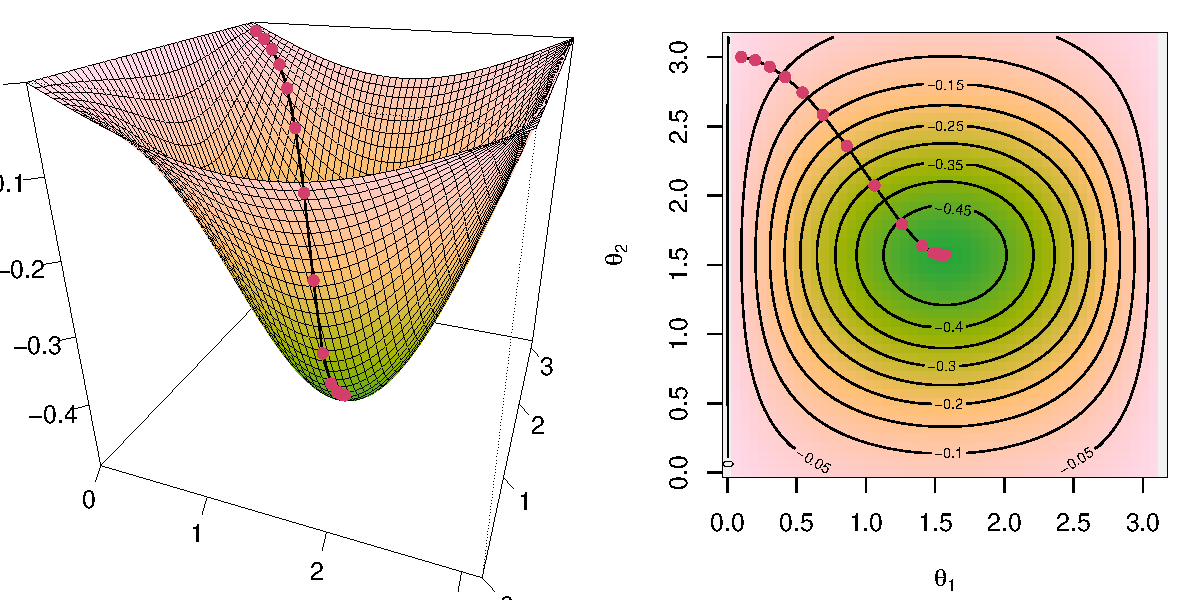
\includegraphics{figure_man/hill.pdf}}
\end{figure}
% \vspace{0.4 cm}
% "Walking down the hill, towards the valley."
% \end{center}
\end{vbframe}
%%%%%%%%%%%%%%%%%%%%%%%%%%%%%%%%%%%%%%%%%%%%%%%%%%%%%%%%%%%%%%%%%%

\begin{vbframe}{Gradient Descent and Optimality}

\begin{minipage}{0.45\textwidth}
    \begin{small}
    \begin{itemize}
      \item GD is a greedy algorithm: In every iteration, it makes locally optimal moves.
      \vspace*{2mm}
      \item If $\riske(\thetab)$ is \textbf{convex} and \textbf{differentiable}, and its gradient is Lipschitz continuous, GD is guaranteed to converge to the global minimum (for small enough step-size).  
      \vspace*{2mm}
    \item However, if $\riske(\thetab)$ has multiple local optima and/or saddle points, GD might only converge to a stationary point (other than the global optimum), depending on the starting point. 
    \end{itemize}
    \end{small}
  \end{minipage}\hfill
  \begin{minipage}{0.5\textwidth}
    \begin{figure}
      \centering
        \scalebox{1}{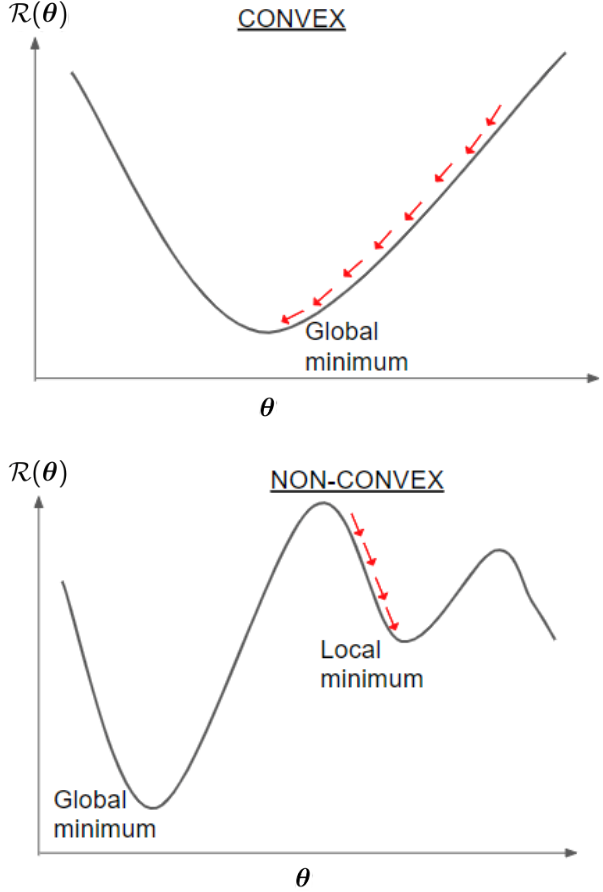
\includegraphics{figure/gdes3.png}}
    \end{figure}
  \end{minipage}  

  \framebreak 

  \textbf{Note: } It might not be that bad if we do not find the global optimum:  

  \begin{itemize}
    \item We don't optimize the (theoretical) risk, but only an approximate version, i.e. the empirical risk. 
    \item For very flexible models, aggressive optimization might overfitting. 
    \item Early-stopping might even increase generalization performance. 
  \end{itemize}

\end{vbframe}

%%%%%%%%%%%%%%%%%%%%%%%%%%%%%%%%%%%%%%%%%%%%%%%%%%%%%%%%%%%%%%%%%%

\begin{vbframe}{Learning rate}

The step-size $\alpha$ plays a key role in the convergence of the algorithm.
\lz

If the step size is too small, the training process may converge \textbf{very} slowly (see left image). If the step size is too large, the process may not converge, because it \textbf{jumps} around the optimal point (see right image).

\begin{center}
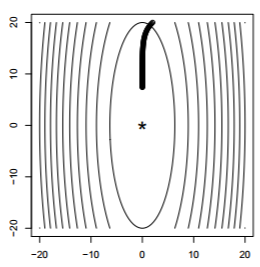
\includegraphics[width = 0.3\textwidth]{figure/stepsize_small.png}~~
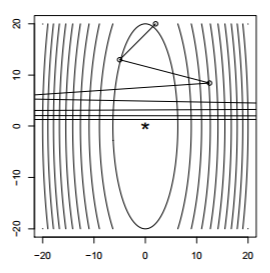
\includegraphics[width = 0.3\textwidth]{figure/stepsize_large.png}
\end{center}

\end{vbframe}

%%%%%%%%%%%%%%%%%%%%%%%%%%%%%%%%%%%%%%%%%%%%%%%%%%%%%%%%%%%%%%%%%%

\begin{vbframe}{Learning Rate}


So far we have assumed a fixed value of $\alpha$ in every iteration:

\vspace*{-0.2cm}
$$\alpha^{[t]} = \alpha \quad \forall t = {\{1, \ldots, T\}}$$

% \textbf{Konvergenz:} Es sei $f:\R^n \to \R$ konvex, differenzierbar und Liptschitz-stetig, d.h. es gibt ein $L > 0$
%
% $$
% \|\nabla f(\bm{x}) - \nabla f(\bm{y})\| \le L\|\bm{x} - \bm{y}\| \quad \text{f?r alle} x, y
%

However, it makes sense to adapt $\alpha$ in every iteration:


\vspace*{-0.1cm}
\begin{center}
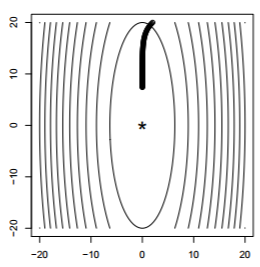
\includegraphics[width = 0.3\textwidth]{figure/stepsize_small.png} ~~~ 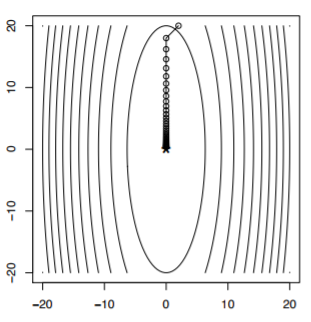
\includegraphics[width = 0.3\textwidth]{figure/stepsize_adaptive.png} \\
\end{center}
\begin{footnotesize}
Steps of gradient descent for $\riske(\thetab) = 10\,\theta_1^2 + 0.5\,\theta_2^2$. Left:  100 steps for with a fixed learning rate. Right:  40 steps with an adaptive learning rate.
\end{footnotesize}


\end{vbframe}
%%%%%%%%%%%%%%%%%%%%%%%%%%%%%%%%%%%%%%%%%%%%%%%%%%%%%%%%%%%%%%%%%%

\begin{vbframe}{Weight Initialization}
\begin{itemize}
\item Weights (and biases) of an NN must be initialized in GD.
\item We somehow must "break symmetry" -- which would happen in full-0-initialization.
    If two neurons (with the same activation) are connected to the same inputs and have the same initial weights, then both neurons will have the same gradient update and learn the same features.
\item Weights are typically drawn from a uniform a Gaussian distribution (both centered at 0 with a small variance).
\item Two common initialization strategies are ’Glorot initialization’ and ’He initialization’ which tune the variance of these distributions based on the topology of the network.
\end{itemize}
\end{vbframe}

%\begin{vbframe}{Weight updates with Backpropagation}
%\begin{itemize}
%\lz
%\item To update each weight $w \in \thetab$ in the network, we need their gradients w.r.t. the empirical risk.
%\lz
%\lz
%\item Since weights are stacked in layers inside the network, we need to repeatedly apply the \enquote{chain rule of calculus}. This process is called \textbf{backpropagation}.
%\lz
%\lz
%\item After obtaining the gradients, the weights can be updated by GD:
%$$\thetab^{[t + 1]} = \thetab^{[t]} - \alpha \cdot \frac{1}{n} \cdot \sumin \nabla_\theta L\left(\yi, f(\xi ~|~ \thetab^{[t]})\right)$$
%\end{itemize}
%\end{vbframe}

%%%%%%%%%%%%%%%%%%%%%%%%%%%%%%%%%%%%%%%%%%%%%%%%%%%%%%%%%%%%%%%%%%

\begin{vbframe}{Stochastic gradient descent}

GD for ERM was: 
$$
  \thetab^{[t + 1]} = \thetab^{[t]} - \alpha \cdot \frac{1}{n} \cdot \sumin \nabla_\theta L\left(\yi, f(\xi ~|~ \thetab^{[t]})\right)
$$
  \begin{itemize}
    \item Using the entire training set in GD to is called \textbf{batch} or \textbf{deterministic} or \textbf{offline training}. This can be computationally costly or impossible, if data does not fit into memory.
    \item \textbf{Idea:} Instead of letting the sum run over the whole dataset, use small stochastic subsets (\textbf{minibatches}), or only a single $\xi$. 
     \item If batches are uniformly sampled from $\Dtrain$, our stochastic gradient is in expectation the batch gradient $\nabla_\theta \risket$.
    \item The gradient w.r.t. a single $\xv$ is fast to compute but not reliable. But its often used in a theoretical analysis of SGD.
    \item[$\to$] We have a \textbf{stochastic}, noisy version of the batch GD.

    % \framebreak 

        % t can be used simply as a computational trick to deal with large data or to operate on real streams of online data in online learning.
    % \item In contrast, the full
    % batch gradient is costly (or even impossible, e.g., when data does not even fit into memory) to compute, particularly in DL, but it averages out all the noise from sub-sampling.
    % \item Minibatches are in between. The batch size decides upon the compromise
    % between speed and averaging (smoothing).
    % \item In summary: SGD computes an unbiased estimate of the gradient by taking the average gradient over a minibatch (or one sample) to update the parameter $\thetab$ in this direction.
    % \item Optimization algorithms that use only a single example at a time are called \textbf{stochastic} or \textbf{online}. This can be used simply as a computational trick to deal with large data or to operate on real streams of online data in online learning.
% Those methods are called \textbf{minibatch} or \textbf{stochastic}.
  \end{itemize}
 
  \framebreak

%%%%%%%%%%%%%%%%%%%%%%%%%%%%%%%%%%%%%%%%%%%%%%%%%%%%%%%%%%%%%%%%%%
 
 SGD on function $1.25(x_1 + 6)^2 + (x_2 - 8)^2$.
 \begin{figure}
    \scalebox{0.8}{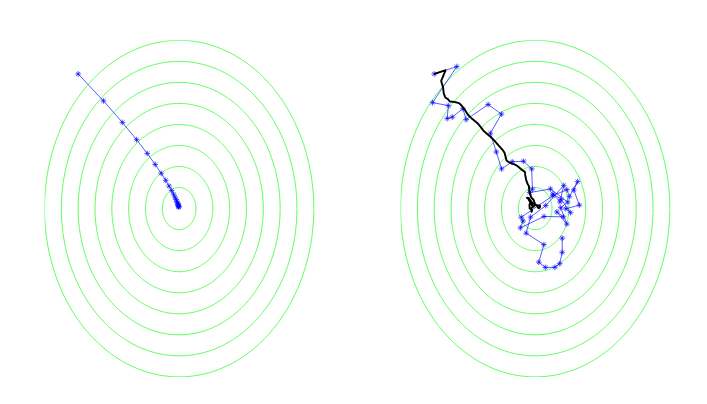
\includegraphics{figure_man/SGD.png}}
    \tiny{\\ Source : Shalev-Shwartz and  Ben-David.
Understanding machine learning: From theory to algorithms. Cambridge University Press, 2014. }
 \caption{Left = GD, right = SGD. The black line is a smoothed $\thetab$.}
 \end{figure}

  \end{vbframe}
  
%%%%%%%%%%%%%%%%%%%%%%%%%%%%%%%%%%%%%%%%%%%%%%%%%%%%%%%%%%%%%%%%%%

% \begin{vbframe}{SGD with Momentum}
% \begin{itemize}
% \item While SGD remains a popular optimization strategy, learning with it can sometimes be slow.
% \item Momentum is designed to accelerate learning, by accumulating an exponentially decaying moving average of past gradients.
% \item Nice tool to get a feel for how momentum works: \url{https://distill.pub/2017/momentum/}
% \end{itemize}
% \begin{figure}
% \centering
% \scalebox{.55}{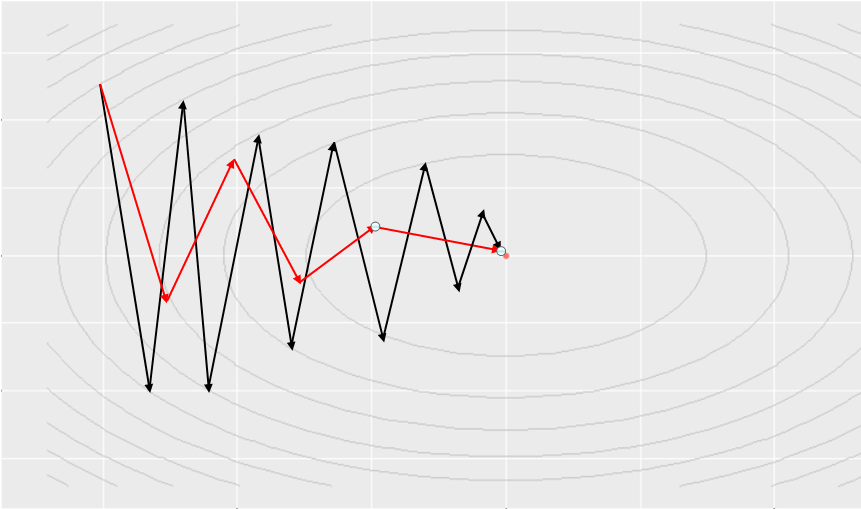
\includegraphics{figure_man/momentum.png}}
% \\GD (black) versus momentum (red) when dealing with ravines
% \end{figure}
% \end{vbframe}

%%%%%%%%%%%%%%%%%%%%%%%%%%%%%%%%%%%%%%%%%%%%%%%%%%%%%%%%%%%%%%%%%%

\begin{vbframe}{Stochastic gradient descent}

  \begin{algorithm}[H]
  \footnotesize
    \caption{Basic SGD pseudo code}
    \begin{algorithmic}[1]
    \State Initialize parameter vector $\thetab^{[0]}$ 
    
    \State $t \leftarrow 0$
    \While{stopping criterion not met}
    \State Randomly shuffle data and partition into minibatches $J_1, ..., J_K$ of size $m$
      \For{$k\in\{1,...,K\}$} 
      \State $t \leftarrow t + 1$ 
      \State Compute gradient estimate with $J_k$: $\hat{g}^{[t]} \leftarrow \frac{1}{m} \sum_{i \in J_k} \nabla_\theta L(\yi, f(\xi ~|~ \thetab^{[t-1]})) $
      \State Apply update: $\thetab^{[t]} \leftarrow \thetab^{[t-1]} - \alpha \hat{g}^{[t]}$
      
      \EndFor
    
        
      \EndWhile
    \end{algorithmic}
  \end{algorithm}
  % \begin{itemize}
  %   \item Thus, what SGD basically does is computing an unbiased estimate of the gradient by taking the average gradients of a minibatch to update the parameter $\thetab$.
  % \end{itemize}
  \begin{itemize}
    \item A full SGD pass over data is an \textbf{epoch}.
        % gradient updates (\textbf{iterations}).
    \item Minibatch sizes are typically between 50 and 1000.
   \end{itemize}
 
\framebreak

%%%%%%%%%%%%%%%%%%%%%%%%%%%%%%%%%%%%%%%%%%%%%%%%%%%%%%%%%%%%%%%%%%
  \begin{itemize}
    \item SGD is the most used optimizer in ML and especially in DL.
        % gradient updates (\textbf{iterations}).
    \item We usually have to add a considerable amount of tricks to SGD to make it really 
        efficient (e.g. momentum). More on this later.
    \item SGD with (small) batches has a high variance, although is unbiased. 
      Hence, the LR $\alpha$ is smaller than in the batch mode.
    % \item SGD with minibatches reduces the variance of the parameter updates and utilizes highly optimized matrix operations to efficiently compute gradients.
  % \item Note: Sometimes, SGD with minibatches is referred to as "Minibatch gradient descent" with the term SGD being reserved for updates using a single example.
    \item When LR is slowly decreased, SGD converges to  local minimum.
    \item Recent results indicate that SGD often leads to better generalization than GD, and may result in indirect regularization.
    % \item Now we know how we can optimize/train a neural network based on the gradient, but how do we compute the gradient? We will learn more about this in the chapter on backpropagation, a method to efficiently compute gradients.
   \end{itemize}
\vspace*{0.5cm}

% \framebreak 

%%%%%%%%%%%%%%%%%%%%%%%%%%%%%%%%%%%%%%%%%%%%%%%%%%%%%%%%%%%%%%%%%%

% \vspace*{0.5cm}
  % \begin{itemize}
  % \end{itemize}
\end{vbframe}

%%%%%%%%%%%%%%%%%%%%%%%%%%%%%%%%%%%%%%%%%%%%%%%%%%%%%%%%%%%%%%%%%%

\endlecture
\end{document}
